%!TEX root = ../dokumentation.tex

\subsection{Technology of HBase}
\label{lblHBaseTechnologies}

In order to understand what the advantages and disadvantages of HBase are, it is important to understand how HBase handles and stores data.
This chapter shall give a brief introduction into the basics of HBase's storage architecture. Therefore, we should define some of the words
we use in this context.

A table is, like in other databases, an ordered set of rows. Unlike other databases, however, HBase does not require a fixed schema for a table.
A row contains \textbf{n} columns which are connected by a so called row key. Since HBase does not support primary keys, the row key is used for the primary
index. Row \textbf{a} of table \textbf{t }and row \textbf{b} of table \textbf{t} do not necessarily need to have the same columns. Row \textbf{a} might have a column \textbf{x} and a column \textbf{y}, while
row \textbf{b} might have column \textbf{z}. At this point, HBase does not require null values for columns for which a row does not provide any data, the columns
just do not exist for this row. \cite{hbase.george.2011}
All columns belong to so called column families. A column family can hold multiple columns and must be defined at the creation time of a table.
The column families and the decision to which family a column should belong are crucial for the performance of HBase. Columns of one column family
are stored sequentially in one file. Therefore, it makes sense to store columns that are regulary accessed together (e.g. name and surname or height and weight)
in one column family to accelerate the reading operations on those columns. \cite{hbase.george.2011}
A column has a name, the qualifier. Together with the row key, the column family name and a timestamp (plus additional flags), it forms the
final key that maps to the value of a specific column in a specific row. The timestamp is necessary because HBase supports multiple versions of a single cell, for example
to have a complete history of the user's last name. \cite{hbase.bertozzi.2012} \cite{hbase.george.2011}

The image \ref{hbase.fig1} on page \pageref{hbase.fig1} illustrates this schema.

\begin{figure}[ht]
	\centering
	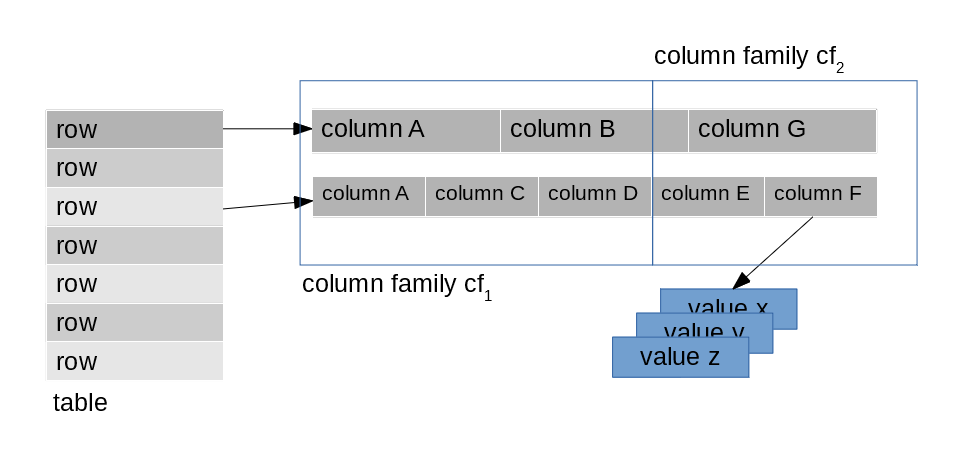
\includegraphics[width=1\textwidth]{images/hbaseTableStructure}
	\caption{structure of a HBase table}
	\label{hbase.fig1}
\end{figure}

The last paragraph already mentioned the storage of HBase. HBase is a so called column oriented database, therefore it does not store the records row by row but
column by column. Since HBase does not have a predefined schema but predefined column families for each table, it stores the values column family by column family.
Each column family is stored in a log structured merge tree, a data structure similar to the b+ trees that are used in traditional RDBMs. The log-structured merge tree
consists of multiple parts of which each is optimized for the storage medium it is stored on. When data is inserted into HBase, the new entry is inserted into a log file first.
After that, the new entry is inserted into an in-memory store. When the in-memory store reaches a certain threshold, it is flushed to the disk as a sorted list of key -> value.
This sorted lists are aranged like typical B-trees with an optimization for sequential disk access. During this process a background worker monitors the new files and merges files
that contain the same column family together after they reach a certain threshold to avoid jumps on the disk. \cite{hbase.george.2011} \cite{hbase.bertozzi.2012}

Although HBase's files are usually stored using the Hadoop File System, HBase itself distributes the data as well to allow for better hardware utilization. The data is distributed
in so called regions. Regions are ranges of rows that are stored together on one server. This must not be confused with the storage of column families: one file contains the data of one
column family, but one column family can be distributed over multiple files. Files that contain the data of the same rows are then stored together in one region. If a region reaches
a certain threshold, the region server splits the region into two regions. \cite{hbase.george.2011}
